% !TEX root = ../main.tex

\subsection{\textsc{Atlas} Humanoid Robot}

\textsc{Atlas} (Fig. \ref{Fig:AtlasDoorFinals}) is an anthropomorphic robot developed by Boston Dynamics, Inc. (BDI). 
Team ViGIR chose to leverage the basic capabilities provided by the Boston Dynamics Application Programming Interface (API).
In the context of this work, we are especially interested in BDI's ``control mode" interface (Fig. \ref{Fig:ControlModeTS}).
The active control mode dictates which joints are controlled by the low-level BDI controllers and which joints we can command.
For example, in \textsc{stand} and \textsc{manipulate} BDI's software handles balancing.

\textsc{Atlas} is equipped with a number of sensors, most notably a Carnegie Robotics Multisense SL\footnote{\scriptsize{\url{http://carnegierobotics.com/multisense-sl}}} mounted as the head.
For the DRC Finals, \textsc{Atlas} was equipped with two Robotiq 3-finger hands,\footnote{\scriptsize{\url{http://robotiq.com/products/industrial-robot-hand}}} providing manipulation capabilities.

\begin{figure}[t]
\centering
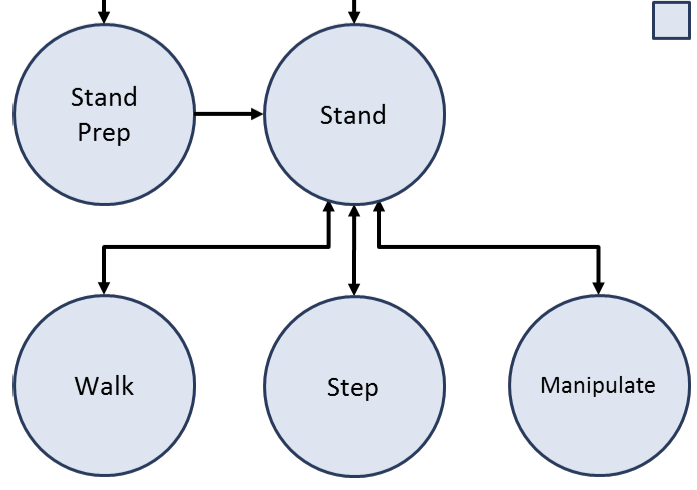
\includegraphics[width=0.99\columnwidth,clip]{./img/control_modes_ts.png}
\caption{Excerpt from the BDI control mode interface.
Some changes between modes (depicted as arrows) are unidirectional while others are bidirectional.
After Team ViGIR's initial checkout, \textsc{Atlas} is in the \textsc{stand\_prep} control mode.
}
\label{Fig:ControlModeTS}
%\vspace{-3 pt}
\end{figure}

\subsection{Team ViGIR's Approach to the DRC Finals}

Team ViGIR based its software on the Robot Operating System (ROS) \cite{ROS2009ICRA, ROS}.
In this section, we highlight some elements of the software's design that are relevant to high-level control and behavior synthesis.
For a complete overview of Team ViGIR's approach, we refer the interested reader to \cite{TeamViGIR2014JFR}.
From this point on, we will refer to \textsc{Atlas} running Team ViGIR's software as the \emph{system}.
\todo[inline, caption = {Replace 2014 JFR with new JFR paper}]{If the new JFR paper is accepted by February, replace this old reference, \cite{TeamViGIR2014JFR}, in the final submission.}

%\subsubsection{Major Software Components}
As mentioned, Team ViGIR uses BDI's control mode interface.
This means that some system capabilities are preconditioned on a certain control mode being active.
For example, in order to execute an arm trajectory, the system must be in \textsc{manipulate}.
In addition, the system's operation has to respect the constraints on the possible control mode changes (Fig. \ref{Fig:ControlModeTS}).

In terms of manipulation, Team ViGIR employs the concept of object templates \cite{Alberto2014Humanoids}.
In brief, the system presents the human operator with perception data, e.g., a point cloud.
Then, the operator detects objects of interest and overlays an object template on top of them.
These templates contain metadata, such as relative robot poses from which the object is reachable, relative pre-grasp and grasp end-effector poses, as well as finger configurations corresponding to different grasps.
In addition, object templates provide manipulation affordances.
For instance, the ``door" template provides affordances such as ``turn (handle) clockwise" and ``push".
\todo[inline, caption = {Improve description of object templates}]{Skim Albert's paper and improve this description of OT.}

\subsubsection*{High-level Control}\label{S:FlexBE}
Team ViGIR's approach to high-level control is especially relevant to this work.
Its corner stone is the Flexible Behavior Engine\footnote{\scriptsize{\url{https://github.com/team-vigir/flexbe_behavior_engine}}} (FlexBE) \cite{Philipp2013Bsc, Philipp2015Msc}, which is a major extension of the SMACH high-level executive \cite{SMACH2010RAM}.

Based on the FlexBE framework, developers create ``state implementations", $\mathsf{s} \in \mathsf{S}$.
These are small, atomic blocks of code that each interact with some primitive, lower-level, system capability, $\mathsf{p} \in \mathsf{P}$.
Furthermore, each state implementation defines a number of outcomes $Out(\mathsf{s})$, e.g. $\{ \mathtt{done}, \mathtt{failed}, \mathtt{aborted} \}$.
The state implementations can be composed to form hierarchical state machines (SM), which encode the logic of execution as well as the flow of data.
State machines also have outcomes themselves.
The top-level state machine will be referred to as a ``behavior".\footnote{\scriptsize{\url{https://github.com/team-vigir/vigir_behaviors}}}
All states of a state machine are parametrized instantiations of the state implementations $\mathsf{S}$.
The composition of new state machines is historically done manually by an expert user.

Finally, composition of behaviors and supervision of their execution takes place in FlexBE's graphical user interface\footnote{\scriptsize{\url{https://github.com/team-vigir/flexbe_chrome_app}}} (GUI).
Figure \ref{Fig:FlexBESM} depicts an example of a high-level behavior designed manually in the FlexBE GUI's editor.

\begin{figure}[t]
\centering
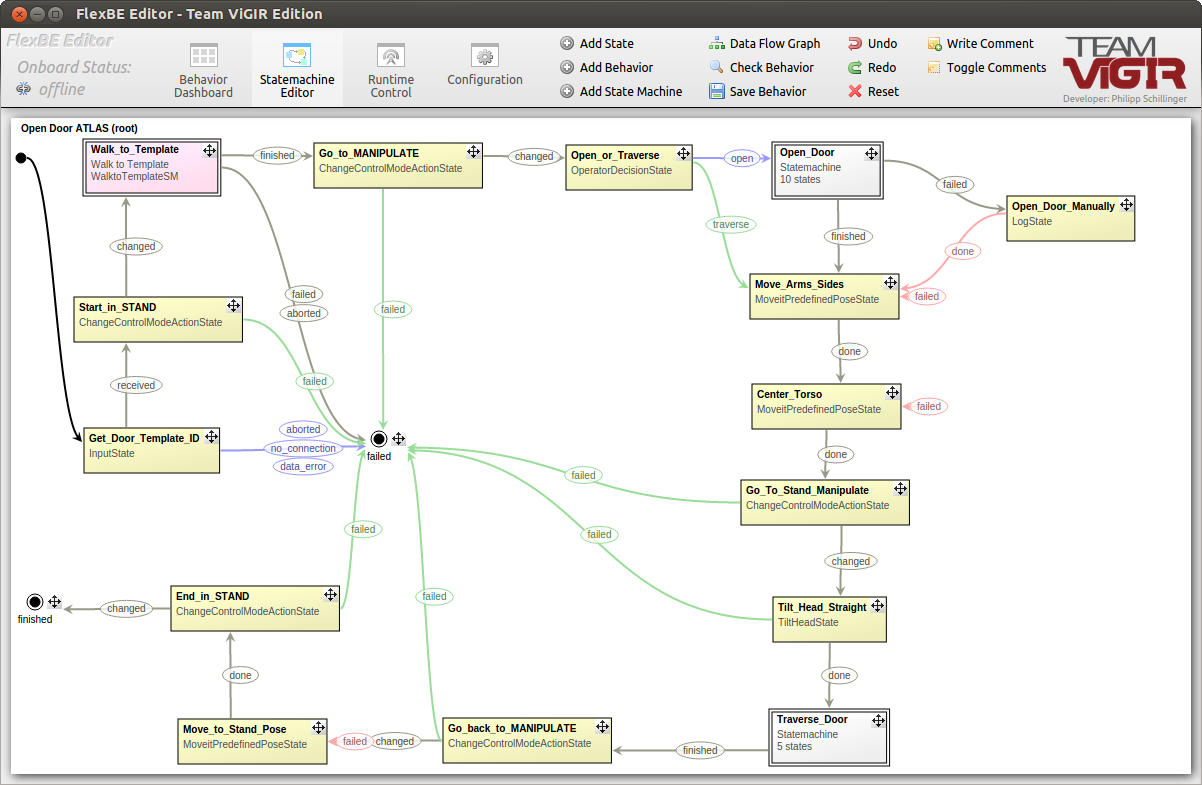
\includegraphics[width=0.99\columnwidth,clip]{./img/behavior_open_door.png}
\caption{A manually designed high-level behavior for carrying out the DRC Finals' ``Door" task.
The initial state is indicated by the black arrow originating from the top left.
The behavior has two outcomes, ``finished" (bottom left) and ``failed" (center).
Yellow states are parametrized state implementations, gray states are state machines, and purple states are other high-level behaviors embedded in this one.
}
\label{Fig:FlexBESM}
\end{figure}

\subsection{Linear Temporal Logic and Reactive LTL Synthesis}\label{S:GR1}

Linear Temporal Logic (\textsc{ltl}) is a formal language that combines Boolean ($\lnot$, $\wedge$, $\lor$) and temporal (next $\LTLX$, until $\mathcal{U}$) operators.
Additional temporal operators, always $\LTLG$, eventually $\LTLF$, can be derived from those.
\textsc{Ltl} formulas are constructed from Boolean atomic propositions $\pi \in AP$.
In the context of our work, the set of atomic propositions, $AP$, consists of propositions controlled by the system, $\mathcal{Y}$, and propositions controlled by the dynamic, and possibly adversarial, environment, $\mathcal{X}$. That is, $AP = \mathcal{X} \cup \mathcal{Y}$.

In order to synthesize \emph{reactive} mission plans in a computationally tractable manner, we use the \textsc{gr(1)} fragment of \textsc{ltl} \cite{piterman_06}.
\textsc{Gr(1)} formulas $\varphi$ have an assume-guarantee structure between the dynamic environment ($e$) and the system ($s$):
%$\varphi = (\varphi_e \Rightarrow \varphi_s)$, where:
%$$\varphi_e = \varphi_e^i \wedge \varphi_e^t \wedge \varphi_e^g, \; \varphi_s = \varphi_s^i \wedge \varphi_s^t \wedge \varphi_s^g,$$
\begin{equation}\label{GR1Formula}
\begin{split}
	\varphi &= (\varphi_e \Rightarrow \varphi_s),\\
	\varphi_e &= \varphi_e^i \wedge \varphi_e^t \wedge \varphi_e^g,\\
	\varphi_s &= \varphi_s^i \wedge \varphi_s^t \wedge \varphi_s^g,
\end{split}
\end{equation}
where the superscript $i$ denotes initial conditions, $t$ safety assumptions/requirements, and $g$ liveness assumptions/requirements (i.e., goals) for $e$ and $s$, respectively. 

\textsc{Gr(1)} synthesis involves setting up a two-player game between $e$ and $s$ \cite{piterman_06}.
If a \textsc{gr(1)} specification $\varphi$ is realizable for $s$, we can extract a finite-state automaton; specifically, a Mealy machine. 
This automaton encodes a strategy for $s$ that guarantees $\varphi_s$ for any evolution of $e$ that satisfies $\varphi_e$.
\todo[inline, caption = {If enough space, define Mealy machine}]{If there's any space left, define the FSA/Mealy machine mathematically. Possibly connect to FlexBE SMs later.}

% END